% ==================================================================================
% CAPÍTULO 2: METODOLOGÍA
% ==================================================================================

\chapter{Metodología}

Este capítulo describe el diseño metodológico de la investigación, detallando el tipo de estudio, enfoque, diseño de investigación, operacionalización de variables, descripción del dataset, técnicas de recolección de datos y procedimientos de análisis. La metodología se fundamenta en los principios de investigación cuantitativa establecidos por \textcite{Hernandez2018}, asegurando rigor científico, reproducibilidad y alineación con el Objetivo General de la investigación: implementar un modelo de Machine Learning supervisado basado en Random Forest para la detección de transacciones fraudulentas y anómalas en pagos digitales de TechSport durante la gestión 2025.

\section{Tipo de Investigación}

Según la taxonomía de \textcite{Hernandez2018}, la presente investigación se clasifica como \textbf{aplicada-tecnológica}, dado que:

\begin{enumerate}
    \item Busca resolver un problema específico identificado en la empresa TechSport: la detección ineficaz de transacciones fraudulentas y anómalas mediante el sistema actual basado en reglas estáticas.

    \item Genera un artefacto tecnológico concreto (modelo de Machine Learning) con aplicación práctica inmediata en el contexto operativo de la organización.

    \item Contribuye al conocimiento aplicado en ingeniería de software y sistemas inteligentes, específicamente en el área de detección de fraude en pagos digitales.

    \item Se alinea directamente con el Área 1.2 Sistemas Inteligentes, línea de investigación de Sistemas Cognitivos, del programa de Maestría en Dirección Estratégica en Ingeniería de Software de la UAGRM.
\end{enumerate}

La investigación aplicada-tecnológica, a diferencia de la investigación básica, no solo busca generar conocimiento nuevo, sino implementar soluciones tecnológicas verificables que aporten valor en contextos reales \parencite{Hernandez2018}.

\section{Enfoque de Investigación}

La investigación adopta un \textbf{enfoque cuantitativo}, fundamentado en el paradigma empírico-analítico (positivista), tal como lo define \textcite{Hernandez2018}. Este enfoque se justifica por las siguientes características del estudio:

\subsection{Características del Enfoque Cuantitativo}

\begin{enumerate}
    \item \textbf{Recolección de datos numéricos:} El dataset histórico de TechSport comprende 25,254,872 transacciones con variables cuantificables (monto, timestamp, frecuencia, etc.) y categóricas (canal de pago, gateway, tipo de transacción).

    \item \textbf{Análisis estadístico riguroso:} Se aplicarán métricas de evaluación cuantitativas (Precision, Recall, F1-Score, AUC-ROC) y análisis de intervalos de confianza mediante bootstrap con 1000 muestras.

    \item \textbf{Medición objetiva de variables:} Tanto la Variable Dependiente (transacciones fraudulentas y anómalas) como la Variable Independiente (modelo de Machine Learning) se operacionalizan mediante indicadores medibles y verificables.

    \item \textbf{Hipótesis cuantificables:} Las hipótesis planteadas contienen valores numéricos específicos que permiten su contrastación empírica (F1-Score $\geq$ 85\%, Recall $\geq$ 90\%, Precision $\geq$ 80\%).

    \item \textbf{Proceso secuencial deductivo:} La investigación sigue una secuencia lógica: problema $\rightarrow$ marco teórico $\rightarrow$ hipótesis $\rightarrow$ recolección de datos $\rightarrow$ análisis $\rightarrow$ conclusiones.

    \item \textbf{Generalización de resultados:} Los hallazgos obtenidos con el dataset de TechSport (74.60\% de cobertura poblacional) permiten inferencias válidas sobre el desempeño del modelo en el contexto de pagos digitales deportivos.
\end{enumerate}

\section{Diseño de Investigación}

\subsection{Diseño Cuasiexperimental Retrospectivo}

El diseño de esta investigación se clasifica como \textbf{cuasiexperimental retrospectivo con evaluación absoluta}, siguiendo la taxonomía de diseños no experimentales de \textcite{Hernandez2018}. Esta clasificación se fundamenta en el análisis crítico de los criterios que definen un diseño experimental verdadero.

\subsubsection{Justificación del Diseño Cuasiexperimental}

Según \textcite{Hernandez2018}, un diseño experimental verdadero requiere tres condiciones:

\begin{table}[H]
\centering
\caption{Análisis de Cumplimiento de Criterios de Diseño Experimental}
\label{tab:experimental_criteria}
\begin{tabular}{@{}p{0.35\textwidth}p{0.15\textwidth}p{0.40\textwidth}@{}}
\toprule
\textbf{Criterio Experimental} & \textbf{¿Cumple?} & \textbf{Justificación} \\
\midrule
Manipulación de variable independiente & Sí & Se implementa el modelo de ML como intervención experimental \\
\midrule
Asignación aleatoria de grupos & No & Se utilizan datos históricos ya ocurridos, sin asignación controlada \\
\midrule
Control del ambiente en tiempo real & No & No hay implementación en producción durante el estudio \\
\midrule
Medición antes-después en tiempo real & No & Análisis retrospectivo de transacciones pasadas \\
\bottomrule
\end{tabular}
\end{table}

Dado que se cumplen parcialmente los criterios (manipulación de VI, pero no asignación aleatoria ni control temporal), el diseño se clasifica como \textbf{cuasiexperimental}.

\subsubsection{Componente Retrospectivo del Diseño}

El diseño es \textbf{retrospectivo} porque:

\begin{itemize}
    \item Los datos analizados corresponden a transacciones ya ocurridas en el periodo 2024-2025.
    \item El etiquetado de las transacciones (fraudulentas vs. legítimas) fue realizado previamente por el equipo de contabilidad de TechSport mediante chargebacks confirmados, disputas resueltas y revisión manual.
    \item No se recolectan datos de manera prospectiva durante la ejecución del estudio.
\end{itemize}

\subsubsection{Evaluación Absoluta (Sin Comparación con Sistema Actual)}

La investigación NO incluye comparación directa con el sistema actual de reglas estáticas debido a:

\begin{enumerate}
    \item \textbf{Falta de acceso a las reglas exactas del sistema:} No se dispone de documentación completa de los umbrales y condiciones booleanas implementadas en el sistema actual.

    \item \textbf{Imposibilidad de reproducir predicciones del sistema actual:} Sin las reglas exactas, no es posible calcular métricas comparables (F1-Score, Precision, Recall) del baseline.

    \item \textbf{Estrategia alternativa de validación:} El modelo de ML propuesto se evalúa mediante:
    \begin{itemize}
        \item Métricas absolutas sobre el test set temporal (transacciones 2025)
        \item Comparación con benchmarks de literatura científica \parencite{Hafez2025}
        \item Intervalos de confianza del 95\% mediante bootstrap
    \end{itemize}
\end{enumerate}

Esta estrategia se alinea con el \textbf{Objetivo Específico 4}: ``Evaluar el desempeño del modelo de Machine Learning mediante métricas de clasificación [\ldots] comparándolo con benchmarks reportados en literatura científica''.

\subsection{Esquema del Diseño Cuasiexperimental}

El diseño se representa mediante el siguiente diagrama:

\begin{figure}[H]
\centering
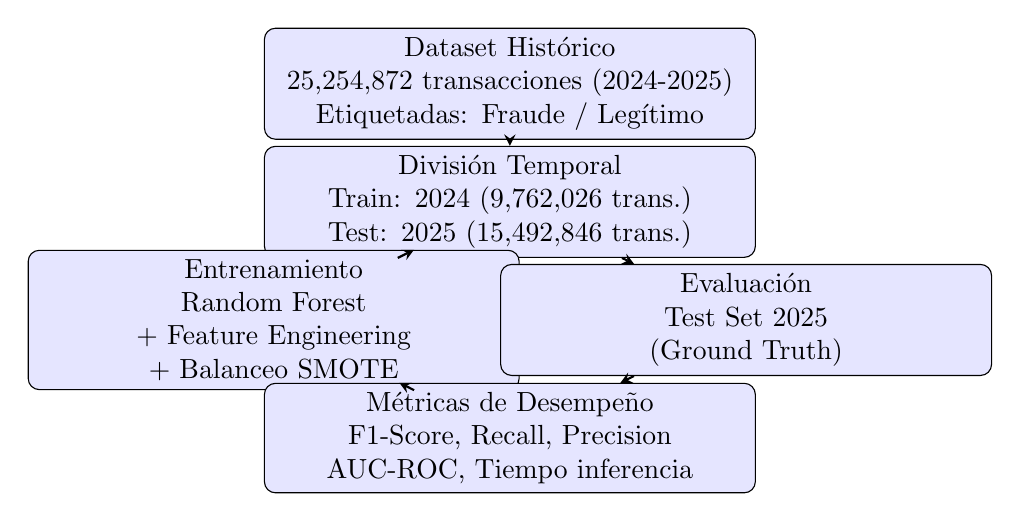
\begin{tikzpicture}[
    node distance=1.5cm,
    block/.style={rectangle, draw, fill=blue!10, text width=6cm, text centered, rounded corners, minimum height=1cm},
    arrow/.style={thick, ->, > = stealth}
]
    \node [block] (dataset) {Dataset Histórico\\25,254,872 transacciones (2024-2025)\\Etiquetadas: Fraude / Legítimo};

    \node [block, below of=dataset] (split) {División Temporal\\Train: 2024 (9,762,026 trans.)\\Test: 2025 (15,492,846 trans.)};

    \node [block, below of=split, xshift=-3cm] (train) {Entrenamiento\\Random Forest\\+ Feature Engineering\\+ Balanceo SMOTE};

    \node [block, below of=split, xshift=3cm] (test) {Evaluación\\Test Set 2025\\(Ground Truth)};

    \node [block, below of=train, xshift=3cm] (metrics) {Métricas de Desempeño\\F1-Score, Recall, Precision\\AUC-ROC, Tiempo inferencia};

    \draw [arrow] (dataset) -- (split);
    \draw [arrow] (split) -- (train);
    \draw [arrow] (split) -- (test);
    \draw [arrow] (train) -- (metrics);
    \draw [arrow] (test) -- (metrics);
\end{tikzpicture}
\caption{Esquema del Diseño Cuasiexperimental Retrospectivo con Validación Temporal}
\label{fig:research_design}
\end{figure}

\subsection{Alcance de la Investigación}

Según \textcite{Hernandez2018}, el alcance de este estudio es \textbf{descriptivo-correlacional-comparativo}:

\begin{enumerate}
    \item \textbf{Descriptivo (alineado con OE2):}
    \begin{itemize}
        \item Describe las características del dataset histórico de TechSport (distribución de fraudes, volumen por canal, patrones temporales).
        \item Caracteriza los tres tipos principales de fraude identificados: tarjetas robadas/clonadas, transacciones duplicadas sospechosas y comportamientos anómalos.
        \item Documenta el proceso de etiquetado realizado por el equipo de contabilidad (criterios, tiempo de etiquetado 0-5 meses).
    \end{itemize}

    \item \textbf{Correlacional:}
    \begin{itemize}
        \item Establece relaciones entre features transaccionales (monto, frecuencia, geolocalización, canal) y la probabilidad de fraude.
        \item Analiza la importancia relativa de cada feature mediante Random Forest feature importance.
        \item Identifica correlaciones multivariadas mediante análisis de matriz de correlación de Pearson.
    \end{itemize}

    \item \textbf{Comparativo (alineado con OE4):}
    \begin{itemize}
        \item Compara el desempeño del modelo Random Forest implementado con benchmarks reportados en literatura científica del periodo 2020-2025.
        \item Cuantifica robustez mediante intervalos de confianza del 95\%.
    \end{itemize}
\end{enumerate}

\textbf{Nota:} El estudio NO es explicativo-causal, ya que no busca establecer relaciones de causa-efecto entre variables independientes del fraude (eso correspondería a criminología), sino evaluar qué tan bien un modelo de ML detecta fraudes ya ocurridos.

\section{Operacionalización de Variables}

La operacionalización de variables transforma conceptos abstractos en indicadores medibles y observables \parencite{Hernandez2018}. Esta sección detalla la \textbf{Variable Madre} (Dependiente), la Variable Independiente y las Variables Intervinientes, en completa alineación con el método AQP/CCA.

\subsection{Variable Dependiente: Transacciones Fraudulentas y Anómalas (Variable Madre)}

\textbf{Justificación de la Variable Madre:} Según el método AQP desarrollado en el perfil de tesis, la ``P'' (Problema) identifica ``Transacciones fraudulentas y anómalas en pagos digitales'' como la variable madre del estudio. Esta es la Variable Dependiente que se busca detectar mediante el modelo de ML.

\subsubsection{Definición Conceptual}

Conjunto de transacciones de pago procesadas por TechSport que presentan comportamientos sospechosos, patrones atípicos o características asociadas a actividad fraudulenta, resultando en pérdidas económicas, chargebacks o afectación de la seguridad financiera de la plataforma \parencite{Baesens2015}.

\subsubsection{Definición Operacional}

Transacciones clasificadas como fraudulentas o anómalas según el proceso de etiquetado de TechSport, basado en:

\begin{enumerate}
    \item Chargebacks confirmados por instituciones financieras
    \item Disputas resueltas como fraude
    \item Reportes de usuarios afectados verificados
    \item Revisión manual de transacciones sospechosas por equipo de contabilidad
\end{enumerate}

\textbf{Proceso de etiquetado:}
\begin{itemize}
    \item \textbf{Responsable:} Equipo de contabilidad de TechSport
    \item \textbf{Tiempo de etiquetado:} Entre 0 días (detección inmediata) hasta 5 meses después de la transacción (chargebacks tardíos)
    \item \textbf{Cobertura:} 100\% de las transacciones del dataset están etiquetadas
\end{itemize}

\textbf{Nota metodológica:} El retraso en el etiquetado refleja la naturaleza real del fraude financiero (chargebacks pueden aparecer semanas o meses después). Esto NO constituye data leakage, ya que las features del modelo utilizan exclusivamente información disponible al momento de la transacción.

\subsubsection{Dimensiones e Indicadores}

\begin{table}[H]
\centering
\caption{Operacionalización de la Variable Dependiente (Variable Madre)}
\label{tab:vd_operationalization}
\small
\begin{tabular}{@{}p{0.25\textwidth}p{0.35\textwidth}p{0.30\textwidth}@{}}
\toprule
\textbf{Dimensión} & \textbf{Indicador} & \textbf{Unidad de Medición} \\
\midrule
Clasificación binaria & Transacción fraudulenta (1) o legítima (0) & Categórica binaria \\
\midrule
Tasa de fraude & (Fraudes / Total transacciones) × 100 & Porcentaje (\%) \\
\midrule
Pérdidas económicas & Suma de montos fraudulentos & Dólares (USD) \\
\midrule
Precisión de detección & VP / (VP + FP) × 100 & Porcentaje (\%) \\
\midrule
Sensibilidad (Recall) & VP / (VP + FN) × 100 & Porcentaje (\%) \\
\midrule
F1-Score & 2 × (Precision × Recall) / (Precision + Recall) & Decimal 0-1 \\
\midrule
Tasa de falsos positivos & FP / (FP + VN) × 100 & Porcentaje (\%) \\
\midrule
AUC-ROC & Área bajo curva ROC & Decimal 0-1 \\
\bottomrule
\end{tabular}
\end{table}

\subsection{Variable Independiente: Modelo de Machine Learning Implementado}

\subsubsection{Definición Conceptual}

Algoritmo computacional basado en aprendizaje automático supervisado, capaz de analizar datos históricos de transacciones etiquetadas para identificar patrones asociados a fraude y predecir la probabilidad de que nuevas transacciones sean fraudulentas o legítimas \parencite{Geron2022}.

\subsubsection{Definición Operacional}

Modelo de clasificación binaria (Fraude/No Fraude) entrenado con el dataset histórico de TechSport, que genera un score de riesgo para cada transacción y una clasificación final basada en un umbral optimizado.

\textbf{Especificaciones técnicas (alineadas con OE3):}
\begin{itemize}
    \item \textbf{Algoritmo principal:} Random Forest (sklearn.ensemble.RandomForestClassifier)
    \item \textbf{Estrategia de entrenamiento:} Supervisado con validación temporal
    \item \textbf{Train set:} Transacciones de 2024 (9,762,026 registros)
    \item \textbf{Test set:} Transacciones de 2025 (15,492,846 registros)
    \item \textbf{Balanceo de clases:} Adaptativo (SMOTE o class weights según distribución)
    \item \textbf{Features:} Mínimo 15 features comportamentales
\end{itemize}

\subsubsection{Dimensiones e Indicadores}

\begin{table}[H]
\centering
\caption{Operacionalización de la Variable Independiente}
\label{tab:vi_operationalization}
\small
\begin{tabular}{@{}p{0.30\textwidth}p{0.35\textwidth}p{0.25\textwidth}@{}}
\toprule
\textbf{Dimensión} & \textbf{Indicador} & \textbf{Valor Objetivo} \\
\midrule
Algoritmo seleccionado & Random Forest & Random Forest \\
\midrule
Profundidad máxima & max\_depth (hiperparámetro) & 10-20 \\
\midrule
Número de estimadores & n\_estimators (Random Forest) & 100-500 \\
\midrule
Balance del dataset & Proporción fraude/legítimo post-SMOTE & 50/50 \\
\midrule
Error de entrenamiento & 1 - Accuracy en train set & < 5\% \\
\midrule
Error de validación & 1 - Accuracy en test set & < 10\% \\
\midrule
Tiempo de inferencia & Milisegundos por transacción & < 200 ms \\
\midrule
Tamaño del modelo & Espacio en disco (serializado) & < 500 MB \\
\bottomrule
\end{tabular}
\end{table}

\subsection{Variables Intervinientes}

Variables que pueden influir en la relación entre VI y VD, pero que no son manipuladas directamente en el estudio:

\begin{table}[H]
\centering
\caption{Variables Intervinientes Identificadas}
\label{tab:intervening_vars}
\small
\begin{tabular}{@{}p{0.25\textwidth}p{0.20\textwidth}p{0.45\textwidth}@{}}
\toprule
\textbf{Variable} & \textbf{Tipo} & \textbf{Influencia en VD} \\
\midrule
Canal de pago & Categórica (Web/App/POS) & Cada canal presenta patrones de fraude diferenciados \\
\midrule
Tipo de transacción & Categórica (Reserva/Membresía/Clínica/Recurrente) & Ciertos tipos son más susceptibles a fraude \\
\midrule
Gateway de pago & Categórica (Stripe/CardConnect/Kushki/etc.) & Cada gateway tiene controles anti-fraude propios \\
\midrule
Volumen transaccional & Numérica continua (trans./día) & Mayor volumen puede facilitar fraudes no detectados \\
\bottomrule
\end{tabular}
\end{table}

\section{Descripción del Dataset}

\subsection{Población y Muestra}

\subsubsection{Población Objetivo}

Según el método AQP, la ``Q'' (Quiénes/Qué) identifica: \textbf{Transacciones de pago digitales de TechSport}. Específicamente:

\begin{itemize}
    \item \textbf{Población total:} Todas las transacciones de pago procesadas por TechSport en su plataforma multicanal durante el periodo 2024-2025.
    \item \textbf{Tipo de transacciones:} Reservas deportivas, membresías, clínicas y cargos recurrentes.
    \item \textbf{Canales:} Web, aplicación móvil y puntos de venta (POS).
    \item \textbf{Gateways:} 10+ pasarelas de pago integradas (Stripe, CardConnect, Kushki, AzulPay, RazorPay, BAC, entre otros).
\end{itemize}

\subsubsection{Dataset Utilizado (Censo Histórico)}

El estudio trabaja con un \textbf{censo de transacciones históricas} del periodo 2024-2025, NO con una muestra aleatoria:

\begin{table}[H]
\centering
\caption{Características del Dataset de TechSport}
\label{tab:dataset_characteristics}
\begin{tabular}{@{}lr@{}}
\toprule
\textbf{Característica} & \textbf{Valor} \\
\midrule
Volumen total de transacciones & 25,254,872 \\
Transacciones 2024 (train set) & 9,762,026 \\
Transacciones 2025 (test set) & 15,492,846 \\
Cobertura poblacional & 74.60\% \\
Periodo temporal & Enero 2024 - Diciembre 2025 \\
Canales de pago & Web, App Móvil, POS \\
Gateways integrados & 10+ (Stripe, CardConnect, Kushki, etc.) \\
Métodos de pago & Tarjetas crédito/débito, ACH, Créditos, Wallets \\
\bottomrule
\end{tabular}
\end{table}

\subsubsection{Justificación Metodológica de Representatividad}

Según \textcite{Hernandez2018}, para estudios cuantitativos con poblaciones grandes, un censo o muestra representativa del 70\%+ es adecuada para inferencias válidas. El dataset de TechSport cumple con:

\begin{itemize}
    \item \textbf{Representatividad temporal:} Cubre 2 años completos de operación, incluyendo variaciones estacionales y tendencias de crecimiento.
    \item \textbf{Diversidad de casos:} Incluye transacciones legítimas y fraudulentas etiquetadas en diversos contextos (canales, gateways, tipos de pago).
    \item \textbf{Datos reales de producción:} NO sintéticos, reflejan el comportamiento real del ecosistema de pagos de TechSport.
    \item \textbf{Diversidad geográfica:} Transacciones procesadas desde múltiples países donde opera TechSport.
\end{itemize}

\subsection{Estructura del Dataset}

El dataset original contiene las siguientes variables raw (previo a feature engineering):

\begin{table}[H]
\centering
\caption{Variables Raw del Dataset de TechSport}
\label{tab:raw_variables}
\small
\begin{tabular}{@{}p{0.30\textwidth}p{0.15\textwidth}p{0.45\textwidth}@{}}
\toprule
\textbf{Variable} & \textbf{Tipo} & \textbf{Descripción} \\
\midrule
transaction\_id & String (UUID) & Identificador único de la transacción \\
timestamp & Datetime & Fecha y hora de la transacción (UTC) \\
user\_id & String (UUID) & Identificador del usuario \\
amount & Float & Monto de la transacción (USD) \\
currency & String & Moneda (mayormente USD) \\
payment\_method & Categórica & Tipo de método de pago \\
channel & Categórica & Canal (web, app, pos) \\
gateway & Categórica & Pasarela de pago utilizada \\
transaction\_type & Categórica & Tipo (reserva, membresía, etc.) \\
ip\_address & String (IP) & Dirección IP del origen \\
country\_ip & String & País de la IP \\
card\_country & String & País emisor de la tarjeta \\
is\_fraud & Binaria (0/1) & Etiqueta: 1=Fraude, 0=Legítimo \\
fraud\_confirmed\_date & Datetime & Fecha de confirmación del fraude \\
\bottomrule
\end{tabular}
\end{table}

\section{Técnicas de Recolección de Datos}

\subsection{Fuentes de Datos}

Los datos provienen de tres fuentes primarias del ecosistema tecnológico de TechSport:

\begin{enumerate}
    \item \textbf{Base de datos transaccional (PostgreSQL):} Registros de todas las transacciones procesadas, incluyendo metadatos de timestamp, monto, usuario, gateway y canal.

    \item \textbf{Sistema de gestión de chargebacks:} Información sobre disputas, chargebacks confirmados y resoluciones de fraude proporcionada por instituciones financieras.

    \item \textbf{Logs de auditoría:} Registros de IP, geolocalización, eventos de autenticación y patrones de navegación.
\end{enumerate}

\subsection{Proceso de Etiquetado}

El etiquetado de transacciones fraudulentas (Variable Dependiente) sigue un proceso multi-criterio realizado por el equipo de contabilidad de TechSport:

\begin{figure}[H]
\centering
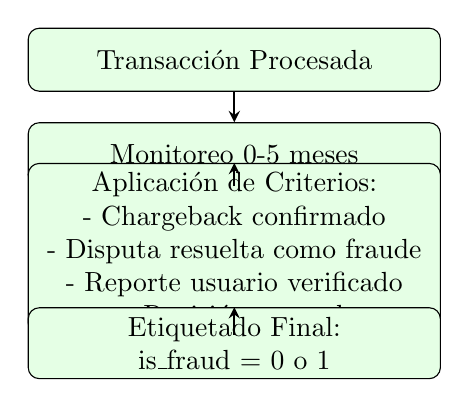
\begin{tikzpicture}[
    node distance=1.2cm,
    block/.style={rectangle, draw, fill=green!10, text width=5cm, text centered, rounded corners, minimum height=0.8cm},
    arrow/.style={thick, ->, > = stealth}
]
    \node [block] (trans) {Transacción Procesada};
    \node [block, below of=trans] (monitor) {Monitoreo 0-5 meses};
    \node [block, below of=monitor] (criteria) {Aplicación de Criterios:\\- Chargeback confirmado\\- Disputa resuelta como fraude\\- Reporte usuario verificado\\- Revisión manual};
    \node [block, below of=criteria] (label) {Etiquetado Final:\\is\_fraud = 0 o 1};

    \draw [arrow] (trans) -- (monitor);
    \draw [arrow] (monitor) -- (criteria);
    \draw [arrow] (criteria) -- (label);
\end{tikzpicture}
\caption{Proceso de Etiquetado de Transacciones Fraudulentas}
\label{fig:labeling_process}
\end{figure}

\textbf{Limitación reconocida:} No se cuenta con métricas de inter-annotator agreement (kappa de Cohen) debido a que el proceso de etiquetado es interno y no fue diseñado originalmente para investigación académica. Sin embargo, el uso de chargebacks confirmados por instituciones financieras proporciona un ground truth confiable.

\section{Técnicas de Procesamiento y Análisis de Datos}

\subsection{Pipeline de Preprocesamiento (Alineado con OE3)}

Según las mejores prácticas de \textcite{Geron2022}, el preprocesamiento del dataset sigue las siguientes etapas:

\subsubsection{Limpieza de Datos}

\begin{enumerate}
    \item \textbf{Manejo de valores faltantes:}
    \begin{itemize}
        \item Variables numéricas: Imputación con mediana (robusto ante outliers)
        \item Variables categóricas: Categoría especial ``UNKNOWN''
        \item Si missing > 40\%: Eliminar variable
    \end{itemize}

    \item \textbf{Detección y tratamiento de outliers:}
    \begin{itemize}
        \item Identificación mediante IQR (Interquartile Range): outliers = valores fuera de $[Q_1 - 1.5 \times IQR, Q_3 + 1.5 \times IQR]$
        \item Estrategia: Winsorización (capear en percentiles 1 y 99) en lugar de eliminación
    \end{itemize}

    \item \textbf{Eliminación de duplicados:}
    \begin{itemize}
        \item Identificación por transaction\_id
        \item Retención de primer registro cronológico
    \end{itemize}
\end{enumerate}

\subsubsection{Feature Engineering (Cumpliendo OE3: Mínimo 15 Features)}

Creación de features comportamentales para capturar patrones de fraude:

\begin{table}[H]
\centering
\caption{Features Engineered (Alineadas con OE3)}
\label{tab:engineered_features}
\scriptsize
\begin{tabular}{@{}p{0.35\textwidth}p{0.55\textwidth}@{}}
\toprule
\textbf{Feature} & \textbf{Descripción y Cálculo} \\
\midrule
monto\_normalizado & (amount - media) / desv\_std (por usuario) \\
\midrule
frecuencia\_24h & Número de transacciones del usuario en últimas 24h \\
\midrule
frecuencia\_7d & Número de transacciones del usuario en últimos 7 días \\
\midrule
monto\_promedio\_historico & Promedio de montos del usuario (hasta t-1) \\
\midrule
ratio\_monto\_vs\_promedio & amount / monto\_promedio\_historico \\
\midrule
tiempo\_desde\_ultima\_trans & Segundos desde última transacción del usuario \\
\midrule
velocidad\_transaccional & Transacciones por hora del usuario \\
\midrule
es\_usuario\_nuevo & 1 si usuario < 30 días desde registro, 0 caso contrario \\
\midrule
distancia\_ip\_tarjeta & Distancia geográfica (km) entre país IP y país tarjeta \\
\midrule
es\_fin\_de\_semana & 1 si día = sábado/domingo, 0 caso contrario \\
\midrule
es\_horario\_nocturno & 1 si hora $\in$ [23:00, 06:00], 0 caso contrario \\
\midrule
hora\_del\_dia & Hora extraída de timestamp (0-23) \\
\midrule
dia\_semana & Día de la semana (0=lunes, 6=domingo) \\
\midrule
monto\_desviacion\_std & (amount - media\_usuario) / std\_usuario \\
\midrule
canal\_encoded & One-hot encoding de canal (web/app/pos) \\
\bottomrule
\end{tabular}
\end{table}

\textbf{Prevención de data leakage:} Todas las features agregadas (promedio histórico, frecuencia, etc.) se calculan usando exclusivamente información disponible ANTES de la transacción actual, mediante ventanas de tiempo con ordenamiento estricto por timestamp.

\subsubsection{División Temporal del Dataset (Alineado con OE3)}

Validación temporal (NO k-fold aleatorio) para respetar la naturaleza cronológica de los datos:

\begin{itemize}
    \item \textbf{Train set:} Todas las transacciones de 2024 (9,762,026 registros)
    \item \textbf{Test set:} Todas las transacciones de 2025 (15,492,846 registros)
\end{itemize}

\textbf{Justificación:} Esta estrategia simula el despliegue real del modelo: entrenamiento con datos históricos (2024), evaluación con datos futuros (2025). Evita el data leakage temporal que ocurriría con k-fold aleatorio \parencite{Geron2022}.

\subsubsection{Balanceo de Clases (Alineado con OE3)}

El desbalanceo de clases será abordado mediante estrategia adaptativa:

\begin{enumerate}
    \item \textbf{Análisis inicial:} Calcular distribución de clases en train set
    \item \textbf{Decisión adaptativa:}
    \begin{itemize}
        \item Si ratio fraude < 1\%: Aplicar SMOTE para generar muestras sintéticas hasta 50/50
        \item Si ratio fraude 1-10\%: Usar class\_weight=``balanced'' en Random Forest
        \item Si ratio fraude > 10\%: No aplicar balanceo adicional
    \end{itemize}
\end{enumerate}

\subsection{Entrenamiento del Modelo (Cumpliendo OE3)}

\subsubsection{Algoritmo Principal: Random Forest}

Implementación mediante scikit-learn 1.3+:

\begin{lstlisting}[style=python, caption=Configuración de Random Forest]
from sklearn.ensemble import RandomForestClassifier

model = RandomForestClassifier(
    n_estimators=300,          # Número de árboles
    max_depth=15,              # Profundidad máxima
    min_samples_split=10,      # Mínimo de muestras para split
    min_samples_leaf=5,        # Mínimo de muestras por hoja
    class_weight='balanced',   # Balanceo automático
    random_state=42,           # Reproducibilidad
    n_jobs=-1                  # Paralelización completa
)
\end{lstlisting}

\subsubsection{Optimización de Hiperparámetros (Alineado con OE3)}

Grid Search sobre espacio de hiperparámetros:

\begin{table}[H]
\centering
\caption{Espacio de Búsqueda de Hiperparámetros}
\label{tab:hyperparameter_space}
\begin{tabular}{@{}lp{0.60\textwidth}@{}}
\toprule
\textbf{Hiperparámetro} & \textbf{Valores a Evaluar} \\
\midrule
n\_estimators & [100, 200, 300, 500] \\
max\_depth & [10, 15, 20, None] \\
min\_samples\_split & [5, 10, 20] \\
min\_samples\_leaf & [2, 5, 10] \\
\bottomrule
\end{tabular}
\end{table}

Criterio de selección: Maximizar F1-Score en validation set.

\subsection{Métricas de Evaluación (Cumpliendo OE4)}

El desempeño del modelo se evaluará mediante las siguientes métricas sobre el test set temporal (transacciones 2025), en completa alineación con el \textbf{Objetivo General} y la \textbf{Hipótesis General}:

\begin{enumerate}
    \item \textbf{Precision:} $\frac{VP}{VP + FP}$ (objetivo: $\geq 80\%$)
    \item \textbf{Recall:} $\frac{VP}{VP + FN}$ (objetivo: $\geq 90\%$, prioritario)
    \item \textbf{F1-Score:} $2 \cdot \frac{\text{Precision} \cdot \text{Recall}}{\text{Precision} + \text{Recall}}$ (objetivo: $\geq 85\%$)
    \item \textbf{AUC-ROC:} Área bajo curva ROC (objetivo: $\geq 0.92$)
    \item \textbf{Tiempo de inferencia:} Milisegundos por transacción (objetivo: $< 200$ ms)
\end{enumerate}

\subsubsection{Intervalos de Confianza (Alineado con OE4)}

Para garantizar robustez estadística, se calcularán intervalos de confianza del 95\% mediante bootstrap:

\begin{itemize}
    \item 1000 muestras bootstrap del test set
    \item Cálculo de F1-Score, Precision, Recall en cada muestra
    \item Estimación de percentiles 2.5\% y 97.5\% para intervalo del 95\%
\end{itemize}

\section{Consideraciones Éticas y de Privacidad}

\subsection{Protección de Datos Personales}

El tratamiento de datos se alinea con principios de GDPR y PCI DSS:

\begin{enumerate}
    \item \textbf{Minimización de datos:} Solo se procesan variables estrictamente necesarias para detección de fraude.
    \item \textbf{Anonimización:} Los user\_id y transaction\_id son pseudoanonimizados mediante hashing SHA-256.
    \item \textbf{Exclusión de datos sensibles:} No se utilizan números de tarjeta completos (PAN), solo primeros 6 dígitos (BIN) y últimos 4 dígitos.
    \item \textbf{Acceso restringido:} Dataset almacenado en infraestructura AWS con cifrado en reposo (AES-256) y en tránsito (TLS 1.3).
\end{enumerate}

\subsection{Uso de Nombre Ficticio}

Por razones de seguridad y confidencialidad empresarial, se utiliza el nombre ficticio ``TechSport'' en lugar del nombre real de la empresa (PlayByPoint), según acuerdo de confidencialidad (NDA) firmado.

\section{Alineación con Objetivos de Investigación}

La metodología descrita responde directamente al Objetivo General y los Objetivos Específicos de la investigación, según lo establece \textcite{Hernandez2018}:

\begin{table}[H]
\centering
\caption{Alineación Metodología - Objetivos - Variable Madre}
\label{tab:methodology_alignment}
\scriptsize
\begin{tabular}{@{}p{0.40\textwidth}p{0.50\textwidth}@{}}
\toprule
\textbf{Objetivo} & \textbf{Componente Metodológico} \\
\midrule
\textbf{Variable Madre (P):} Transacciones fraudulentas y anómalas & Variable Dependiente operacionalizada con 8 indicadores cuantificables \\
\midrule
\textbf{OG:} Implementar modelo ML para detección de fraude (F1 $\geq$ 85\%, Recall $\geq$ 90\%, Precision $\geq$ 80\%) & Diseño cuasiexperimental + Random Forest + Validación temporal + Métricas cuantificables \\
\midrule
\textbf{OE1:} Fundamentación teórica de ML en fraude & Revisión de literatura 2020-2025 + Benchmarks (Capítulo 1) \\
\midrule
\textbf{OE2:} Diagnóstico del sistema actual mediante EDA & Análisis exploratorio del dataset + Caracterización de 3 patrones de fraude + Documentación proceso etiquetado \\
\midrule
\textbf{OE3:} Desarrollo del modelo ML con 15+ features & Pipeline preprocesamiento + Feature engineering (15 features) + Entrenamiento Random Forest + Optimización hiperparámetros + División temporal 2024/2025 \\
\midrule
\textbf{OE4:} Evaluación comparativa con benchmarks & Métricas test set + Comparación con literatura (Hafez 2025) + Intervalos confianza bootstrap 95\% \\
\bottomrule
\end{tabular}
\end{table}

\section{Síntesis Metodológica}

El diseño metodológico de esta investigación se fundamenta en un enfoque cuantitativo con diseño cuasiexperimental retrospectivo, operacionalizando rigurosamente la \textbf{Variable Madre} (transacciones fraudulentas y anómalas) identificada en el método AQP como la Variable Dependiente, y la Variable Independiente (modelo de Machine Learning supervisado basado en Random Forest). La validación temporal del dataset (train: 2024, test: 2025) asegura robustez ante concept drift, mientras que las métricas cuantificables (F1-Score $\geq$ 85\%, Recall $\geq$ 90\%, Precision $\geq$ 80\%) permiten la contrastación empírica de las hipótesis planteadas.

Cada componente metodológico se alinea directamente con los Objetivos Específicos: OE2 (diagnóstico), OE3 (desarrollo con 15+ features), y OE4 (evaluación comparativa con benchmarks de literatura). La metodología cumple con los principios de rigor científico, reproducibilidad y coherencia interna establecidos por \textcite{Hernandez2018}, garantizando que los hallazgos respondan al Objetivo General de la investigación.

\cleardoublepage
